\chapter{How to obtain the CRTM}
%===============================

\section{CRTM ftp download site}
%===============================
The CRTM source code and coefficients, and example programs, are released as compressed tarballs\footnote{A compressed (e.g. gzip'd) tape archive (tar) file.} via the CRTM ftp site:

\hspace{1cm}\texttt{ftp://ftp.emc.ncep.noaa.gov/jcsda/CRTM/}

A snapshot of that site is shown in figure \ref{fig:ftp_site}. Note that the source code and coefficients can be released separately as updates to either one can occur independently of the other. Also note that additional releases, e.g. beta or experimental branches, are also made available on this ftp site.

\begin{figure}[htb]
  \centering
  \includegraphics[scale=0.5]{graphics/Get/CRTM_ftp_site.eps}
  \caption{The CRTM ftp site contents (as on Feb.03, 2009)}
  \label{fig:ftp_site}
\end{figure}

\section{Coefficient Data}
%=========================
The tarball labeled as ``\texttt{Coeffs}'' packages up all the transmittance, spectral, cloud, aerosol, and emissivity coefficient data needed by the CRTM. The Coeffs tarball directory structure is organised by coefficient and format type as shown below,

\begin{alltt}
    CRTM_Coefficients/
     |- SpcCoeff/
     |   |- Big_Endian/
     |   |- Little_Endian/
     |   `- netCDF/
     |- TauCoeff/
     |   |- Big_Endian/
     |   |- Little_Endian/
     |   `- netCDF/
     |- AerosolCoeff/
     |   |- Big_Endian/
     |   |- Little_Endian/
     |   `- netCDF/
     |- CloudCoeff/
     |   |- Big_Endian/
     |   |- Little_Endian/
     |   `- netCDF/
     `- EmisCoeff/
         |- Big_Endian/
         |- Little_Endian/
         `- netCDF/
\end{alltt}
Both big- and little-endian format files are provided to save users the trouble of switching what they use for their system. Planned future updates to the CRTM include changing the CRTM initialisation I/O functions to the netCDF versions so, eventually, only the netCDF datafiles will be provided.

To run the CRTM, all the required coefficient files need to be in the same path (see the  \hyperref[sec:CRTM_Init_interface]{CRTM initialisation function} description) so users will have to move the datafiles as required.


\section{Example Programs}
%=========================
The tarball labeled as ``\texttt{Example\_Code}'' contains two completely independent example programs -- one showing how to call the CRTM Forward model and the other for the K-matrix model. The Example Code tarball directory structure looks like that below, with the example programs higlighted in blue,

\begin{alltt}
    Example_Code/
     |- Coefficient_Data/
     |   |- AerosolCoeff.bin
     |   |- CloudCoeff.bin
     |   |- EmisCoeff.bin
     |   |- amsua_n18.SpcCoeff.bin
     |   |- amsua_n18.TauCoeff.bin
     |   |- hirs4_n18.SpcCoeff.bin
     |   |- hirs4_n18.TauCoeff.bin
     |   |- mhs_n18.SpcCoeff.bin
     |   `- mhs_n18.TauCoeff.bin
     |- Forward/
     |   |- \textcolor{blue}{Example_Forward.f90}
     |   |- Makefile
     |   |- README.FIRST
     |   |- run_Example_Forward.sh*
     |   `- Results/
     |       |- amsua_n18.Forward.output
     |       |- hirs4_n18.Forward.output
     |       `- mhs_n18.Forward.output
     `- K_Matrix/
         |- \textcolor{blue}{Example_K_Matrix.f90}
         |- Makefile
         |- README.FIRST
         |- run_Example_K_Matrix.sh*
         `- Results/
             |- amsua_n18.K_Matrix.output
             |- hirs4_n18.K_Matrix.output
             `- mhs_n18.K_Matrix.output
\end{alltt}

The example programs are written to search for the test coefficient files' (all big-endian) relative location as shown. There are two additional things to note about the example program makefiles,
\begin{itemize}
  \item they assume the CRTM library has already been built (see chapter \ref{sec:build} for how to do that) \emph{and} is in the generic location, \texttt{\$(HOME)/local/CRTM},
  \item \texttt{gfortran} is the default compiler.
\end{itemize}
You should modify the example code makefiles for your own system. Other compiler switches are provided in the makefile for guidance. 

The shell script files, \texttt{run\_Example\_Forward.sh} and \texttt{run\_Example\_K\_Matrix.sh}, run the example programs as well as compare their output to that supplied in the \texttt{Results} directory.




